\documentclass[a4paper,twocolumn,floatfix]{revtex4-1}
\usepackage{t1enc}
\usepackage[T1]{fontenc}
\usepackage{ulem}
\usepackage{import}
\usepackage{amsmath}
\usepackage{amssymb}
\usepackage{paralist}
\usepackage{booktabs}
\usepackage[version=3]{mhchem}
\usepackage{wrapfig}
\usepackage{pifont}
\usepackage{mathrsfs}
\usepackage{tikz}
\usepackage{xcolor}
\usepackage{color}
\usepackage{enumitem}
\usepackage{datetime}
\usepackage{textcomp}
\usepackage{relsize}
\usepackage{pgfplotstable}
%\setlist{noitemsep}
%\usepackage{lineno}
%\linenumbers

\usepackage{pgfplots}
\pgfplotsset{compat=newest}
\usepgfplotslibrary{units}
\usetikzlibrary{pgfplots.units} 
\usetikzlibrary{calc} 
\usepgfplotslibrary{groupplots}
\usepackage{siunitx}
%\DeclareSIUnit\molar{\mole\per\cubic\deci\metre}
%\DeclareSIUnit\textsc{M}{\textsc{M}}

\usepackage{hyperref}
\hypersetup{
 colorlinks=false,
 hidelinks=true,
}

\newcommand{\Figure}[1]{Fig.~\ref{#1}}
\newcommand{\Equation}[1]{Eqn.~\ref{#1}}
\newcommand{\Table}[1]{Tbl.~\ref{#1}}
\newcommand{\Section}[1]{Sec.~\ref{#1}}
\newcommand{\Chapter}[1]{Ch.~\ref{#1}}
\newcommand{\Appendix}[1]{Appendix~\ref{#1}}

% use roman type for natural base e and sqrt(-1)
\newcommand{\me}{{\mathrm{e}}}
\newcommand{\mi}{{\mathrm{i}}}

\definecolor{colora}{RGB}{24,90,169}
\definecolor{colorb}{RGB}{238,46,47}
\definecolor{colorc}{RGB}{0,140,72}
\definecolor{colord}{RGB}{244,125,35}
\definecolor{colore}{RGB}{61,90,153}
\definecolor{colorf}{RGB}{102,44,145}

\definecolor{tangoorange}{RGB}{245,121,0}

\newcommand{\todo}[1]{%
\textcolor{tangoorange}{#1}
}

\import{colors/}{colors}

% color cycle thing
\pgfplotscreateplotcyclelist{cbDark27qual}{
 {color=colora,mark=x},
 {color=colorb,mark=+},
 {color=Dark27qual3,mark=o},
 {color=Dark27qual4,mark=x},
 {color=Dark27qual5,mark=x},
 {color=Dark27qual6,mark=x},
 {color=Dark27qual7,mark=x},
}


\begin{document}
\thispagestyle{empty}
\pgfplotsset{
 minor tick num=3,
 footnotesize,
 every
 axis/.style={height=100pt,width=190pt,
  thick,
 %enlargelimits=false,
 %xmin=-1e-6,xmax=2.5e-6,
 %ymin=-1,ymax=1,
 xlabel=contact surface density $A_c$,
 x unit=-,
 ylabel={$\Delta\!f$, $\Delta\Gamma$},
 y unit = \si{\hertz},
 restrict x to domain = {-0.3:0.4},
 max space between ticks=30pt,
 mark size=1.5pt,
 ylabel style={ yshift=-5pt, },
 %scaled x ticks = {real:1e-6},
 %xticklabel style={/pgf/number format/fixed},
 %every x tick scale label/.style={color=white,},
 legend columns=-1,
 legend style={font=\footnotesize},
 legend style={draw=none,font=\tiny},
 legend image post style={xscale=0.5},
 legend pos = south west,
 },
}
 \begin{tabular}{ll}
\begin{tikzpicture}[baseline, trim axis left]
 \pgfplotstableread{data/multisweep-cells.dat}{\datatable}
 \begin{axis}[
   x unit = {},
   xlabel = {},
   ymax=1,
   ymin=-1,
  ]
  \addplot [smooth,mark=, color=colora,] table [ y expr=\thisrowno{1} ] {\datatable};
  \addplot [smooth,mark=, color=colorb,densely dashdotted] table [ y expr=\thisrowno{2} ] {\datatable};
  \addplot [color=gray,dashed,semithick] coordinates {(0,-1) (0,1)};
  \node[anchor=north west] at (yticklabel* cs:1) {(a)};
  \legend{$\Delta\!f$,$\Delta\Gamma$}
 \end{axis}
 \end{tikzpicture}
 &
 \hspace{-0.25cm}
 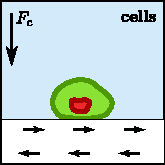
\includegraphics[height=55pt,keepaspectratio]{images/cells.pdf}
\\
\begin{tikzpicture}[baseline,trim axis left]
 \pgfplotstableread{data/multisweep-agarose.dat}{\datatable}
 \begin{axis}[
   x unit = {},
   xlabel = {},
   ymax=1,
   ymin=-1,
  ]
  \addplot [smooth,mark=, color=colora,] table [ y expr=\thisrowno{1} ] {\datatable};
  \addplot [smooth,mark=, color=colorb,densely dashdotted] table [ y expr=\thisrowno{2} ] {\datatable};
  \addplot [color=gray,dashed,semithick] coordinates {(0,-1) (0,1)};
  \node[anchor=north west] at (yticklabel* cs:1) {(b)};
  \legend{$\Delta\!f$,$\Delta\Gamma$}
 \end{axis}
 \end{tikzpicture}
 &
 \hspace{-0.25cm}
 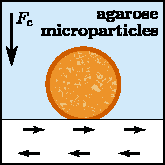
\includegraphics[height=55pt,keepaspectratio]{images/agarose.pdf}
 \\
\begin{tikzpicture}[baseline,trim axis left]
 \pgfplotstableread{data/multisweep-lysozyme.dat}{\datatable}
 \begin{axis}[
   ymin=-1.1,
   ymax=1,
  ]
  \addplot [smooth,mark=, color=colora,] table [ y expr=\thisrowno{1} ] {\datatable};
  \addplot [smooth,mark=, color=colorb,densely dashdotted] table [ y expr=\thisrowno{2} ] {\datatable};
  \addplot [color=gray,dashed,semithick] coordinates {(0,-1) (0,1)};
  \node[anchor=north west] at (yticklabel* cs:1) {(c)};
  \legend{$\Delta\!f$,$\Delta\Gamma$}
  \end{axis}
 \end{tikzpicture}
 &
 \hspace{-0.25cm}
 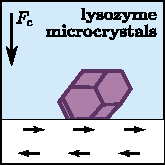
\includegraphics[height=55pt,keepaspectratio]{images/lysozyme.pdf}
\end{tabular}
\end{document}
